%%--------- Comandos especiales
\newcommand{\vecr}{\mathbf{r}}
\newcommand{\veck}{\mathbf{k}}
\newcommand{\nnet}{N_{\theta}(\mathbf{r})}
%%
\chapter{Solución a la ecuación de Ornstein-Zernike usando redes neuronales} % Main chapter title

\label{Cap3} % Change X to a consecutive number; for referencing this chapter elsewhere, use \ref{ChapterX}

%----------------------------------------------------------------------------------------
%	SECTION 1
%----------------------------------------------------------------------------------------

Las \emph{redes neuronales} fungen como aproximadores universales~\cite{hornikMultilayerFeedforwardNetworks1989, hornikApproximationCapabilitiesMultilayer1991, cybenkoApproximationSuperpositionsSigmoidal1989},
y como tal pueden ser utilizadas para aproximar cualquier función continua para un determinado tipo de arquitectura.
En particular, se espera que una red neuronal pueda servir como paramatrización de la
función puente en la condición de cerradura de la ecuación de OZ, y así evitar escoger
una aproximación en especial, y dejar que la red neuronal tome la forma necesaria
para resolver la ecuación integral.

En este capítulo se detalla la metodología creada y los fundamentos matemáticos bajo los
cuales se puede hacer uso de redes neuronales para resolver la ecuación de OZ.
Se comparan estos resultados con los obtenidos con simulación por computadora.
En el apéndice se describe la solución general a la ecuación de OZ, mientras que
en este capítulo se detalla su modificación para emplear redes neuronales.

\section{Parametrización de la función puente}

La ecuación de Ornstein-Zernike está dada por

\begin{subequations}
    \begin{align*}
         & c(\vecr) = h(\vecr) +
        n \int_{V}
        c(\vecr^{\prime})
        h(\lvert \vecr - \vecr^{\prime} \rvert)
        d\vecr^{\prime} \label{eq:oz1} \\
         & c(\vecr)
        = \exp{\left[
                -  \beta u(\vecr)
                +  \gamma(\vecr)
                + B(\vecr)
                \right]} -
        \gamma(\vecr)
        - 1
    \end{align*}
\end{subequations}

con la notación ya conocida para esta ecuación.

Sea $\nnet$ una red neuronal con pesos $\theta$. Se propone que
$\nnet$ reemplace a la función puente $B(\vecr)$ en la ecuación
anterior tal que ahora se tiene la siguiente expresión para la cerradura

\begin{equation}
    c(\vecr) = \exp{\left[
            -  \beta u(\vecr)
            +  \gamma(\vecr)
            + \nnet
            \right]} -
    \gamma(\vecr)
    - 1 ,
    \label{eq:parametrizacion}
\end{equation}

y la ecuación de OZ queda de la misma forma.
Se pretende trabajar a partir de esta hipótesis donde la función puente
pueda tomar cualquier valor en particular que permita la solución de la
ecuación de OZ.

%----------------------------------------------------------------------------------------
%	SECTION 2
%----------------------------------------------------------------------------------------

\section{Esquema de entrenamiento}
Ahora que se tiene la parametrización, se debe desarrollar una forma para ajustar los
pesos de la red neuronal $\nnet$, y que al mismo tiempo permita la solución
de la ecuación de OZ.

\subsection{Función de costo}
Para crear un esquema de entrenamiento se requiere primero de una \textbf{función de costo}
que sea utilizada para generar información del ajuste necesario de los pesos $\theta$.
Tomando en cuenta que el esquema iterativo de Piccard crea una sucesión de funciones
estimadas $\{\gamma_1(\vecr), \gamma_2(\vecr), \dots, \gamma_n(\vecr)\}$, se propone que la función de costo
sea

\begin{equation}
    J(\theta) = \left[\gamma_{n}(\vecr; \theta) - \gamma_{n-1}(\vecr; \theta) \right]^2
    \label{eq:costo}
\end{equation}

donde $\gamma_{n}(\vecr; \theta)$ es la enésima función estimada de $\gamma(\vecr)$
mediante el método iterativo. La notación $\gamma(\vecr; \theta)$ indica que depende
implícitamente de los pesos de la red neuronal, como se puede ver en el ecuación~\eqref{eq:parametrizacion}.
Esto significa que si los pesos de $\nnet$ cambian, entonces la función $\gamma$ debe cambiar.
Sin embargo, esto no significa que $\gamma$ depende \emph{directamente} de los pesos.

\subsection{Problema de optimización}
Usando la función de costo~\eqref{eq:costo} ahora se puede plantear un problema de optimización
que permita el ajuste de los pesos de $\nnet$.

El problema de optimización en este caso es \emph{sin restricciones} y está
definido de la siguiente forma

\begin{equation}
    \begin{aligned}
         & \underset{\theta}{\text{min}}
         & & J(\theta)
    \end{aligned}
    \label{eq:optimizacion}
\end{equation}

Esto significa que buscamos los parámetros óptimos $\theta^*$ que minimicen la diferencia
entre las iteraciones calculadas de las funciones $\gamma(\vecr; \theta).$
Este problema de optimización se puede resolver de forma iterativa, al mismo tiempo que
se resuelve la ecuación de OZ.

\subsection{Actualización de pesos}
El método iterativo empleado está basado en la técnica de \emph{descenso de gradiente}
para actualizar los pesos de la red neuronal.
Esto significa que en general, una regla de actualización está dada por una expresión
semejante a la siguiente

\begin{equation}
    \theta_{n+1} = \theta_n - \nabla_{\theta} J(\theta) .
    \label{eq:gradiente}
\end{equation}

% TODO: Cambiar el nombre del apéndice
Independientemente de la expresión de la actualización de los pesos, este cálculo
requiere de la información del gradiente de la función de costo respecto a los pesos,
$\nabla_{\theta} J(\theta)$.
Para este caso en particular, el cálculo detallado del gradiente se describe en el apéndice.
Una vez que se tiene esta información, lo que resta es construir un algoritmo que use
este esquema de entrenamiento y que resuelva la ecuación de OZ.

\subsection{Solución a la ecuación de Ornstein-Zernike con redes neuronales}
Con todos los elementos necesarios, se puede entonces definir el esquema general para
la solución a la ecuación de Ornstein-Zernike usando redes neuronales.

Para resolver la ecuación de OZ con la parametrización~\eqref{eq:parametrizacion} se tienen lo siguientes pasos:

\begin{enumerate}
    \item Dado el potencial de interación $u(\vecr)$, se emplea la ecuación~\eqref{eq:parametrizacion} para obtener el valor de $c(\vecr; \theta),$ la cual ahora depende implícitamente de los pesos de $\nnet$. En este paso también se requiere de un valor inicial para $\gamma_{n}(\vecr),$ el cual se inicializa de acuerdo a la metodología de Ng de cinco puntos, descrita en el apéndice. %% TODO: Cambiar el nombre del apéndice
    \item La función $c(\vecr; \theta)$ se transforma mediante la transformada de Fourier, para obtener $\hat{c}(\veck; \theta)$.
    \item Se transforma mediante la transformada de Fourier toda la ecuación de OZ, y se deja en términos de la función $\hat{\gamma}(\veck)$. Usando la información encontrada sobre la función $\hat{c}(\veck; \theta)$, se encuentra una nueva función $\hat{\gamma}_{n+1}(\veck; \theta)$.
    \item Luego, se antitransforma la función $\hat{\gamma}_{n+1}(\veck; \theta)$ para obtener la nueva estimación, $\gamma_{n+1}(\vecr; \theta)$.
    \item Usando ambas estimaciones $\gamma_{n}$ y $\gamma_{n+1}$, se evalúa la función de costo~\eqref{eq:costo} y se realiza el cálculo del gradiente, $\nabla_{\theta} J(\theta)$.
    \item Se actualizan los pesos usando la expresión~\eqref{eq:gradiente}, y se reinicia el proceso. En la siguiente iteración, la función inicial será ahora $\gamma_{n+1}$, para entonces obtener una nueva estimación $\gamma_{n+2}$, y así sucesivamente.
\end{enumerate}

\subsection{Convergencia del entrenamiento}
El procedimiento descrito anteriormente se repite de forma indefinida hasta lograr la 
convergencia, dada por la siguiente expresión

\begin{equation}
    {\lvert \gamma_{n+1} - \gamma_{n} \rvert}^2 \leq \epsilon
    \label{eq:tolerancia}
\end{equation}

donde $\lvert \cdot \rvert$ indica el valor absoluto, y $\epsilon \in [0, 1]$.
En particular, la tolerancia en todos los experimentos realizados fue de
$\epsilon = 1 \times 10^{-5}$.
En otras palabras, se exige a la red neuronal ajustar sus pesos hasta que las estimaciones
sucesivas de las funciones $\gamma$ sean muy semejantes entre sí.

%----------------------------------------------------------------------------------------
%	SECTION 3
%----------------------------------------------------------------------------------------

\section{Resultados}

\begin{figure}
    \centering
    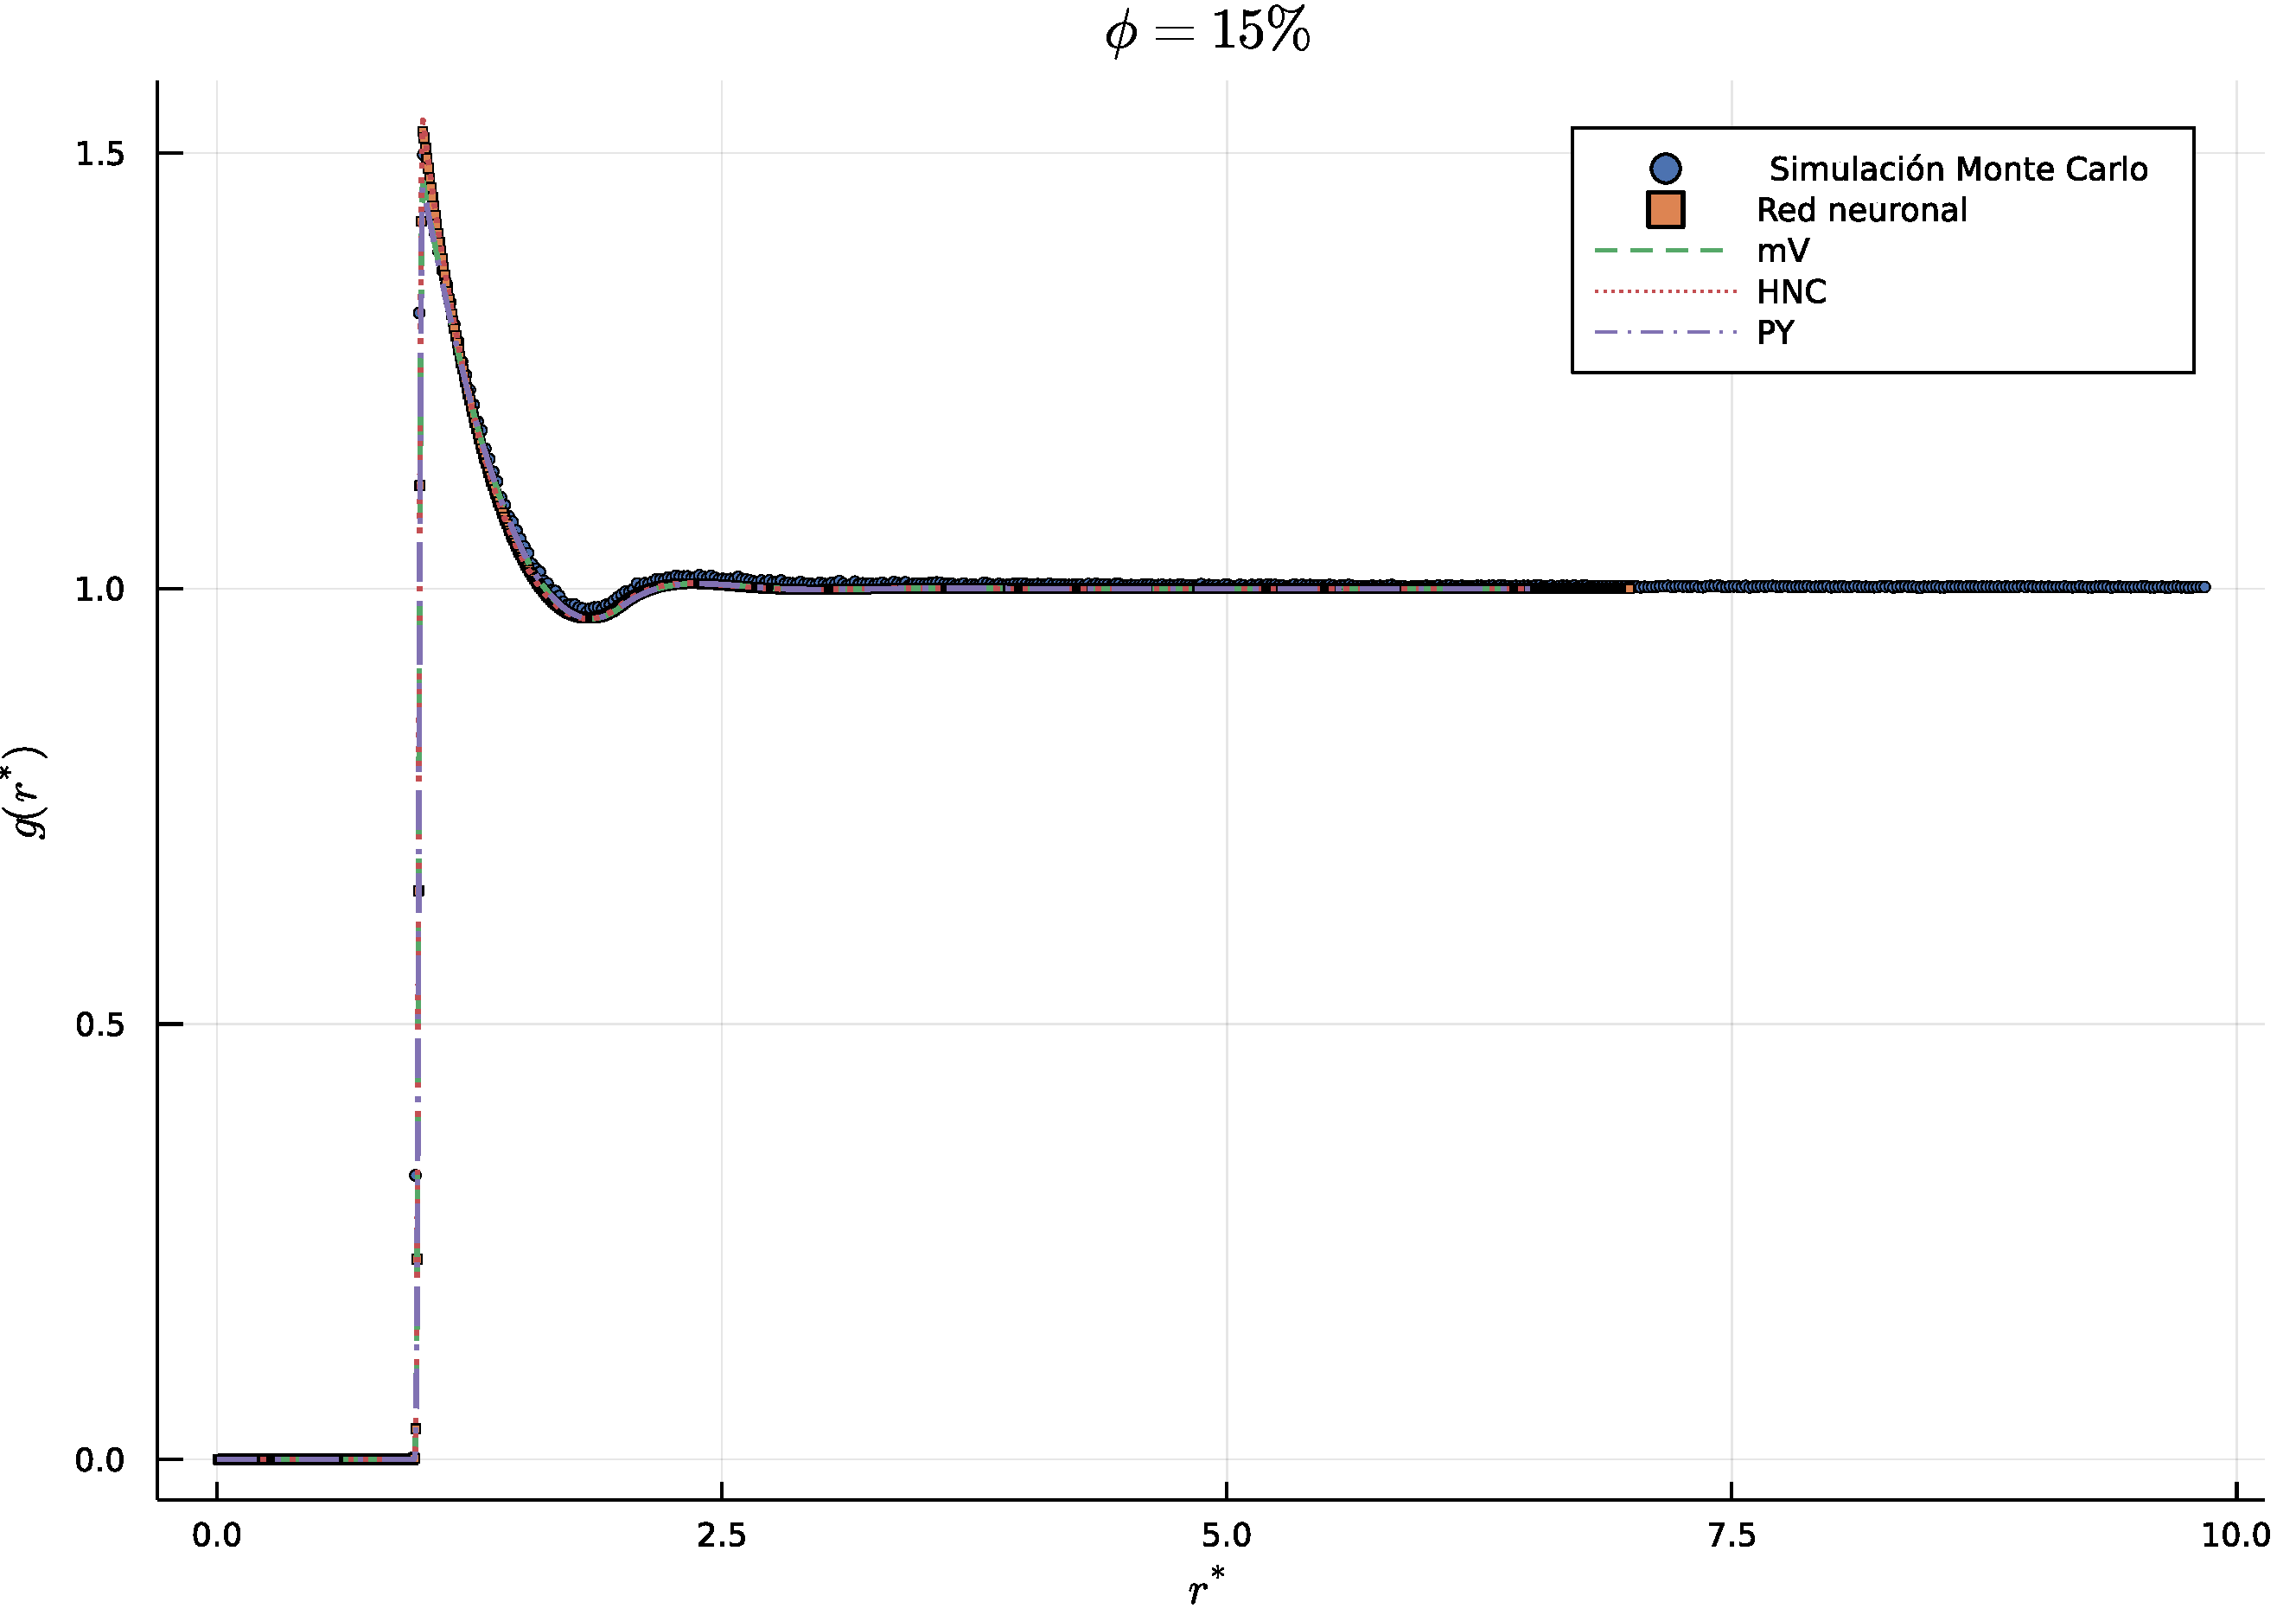
\includegraphics[width=\textwidth]{figuras/capitulo-3/p=0.15.pdf}
    \caption{Una figura.}
    \label{fig:fig1}
\end{figure}

\begin{figure}
    \centering
    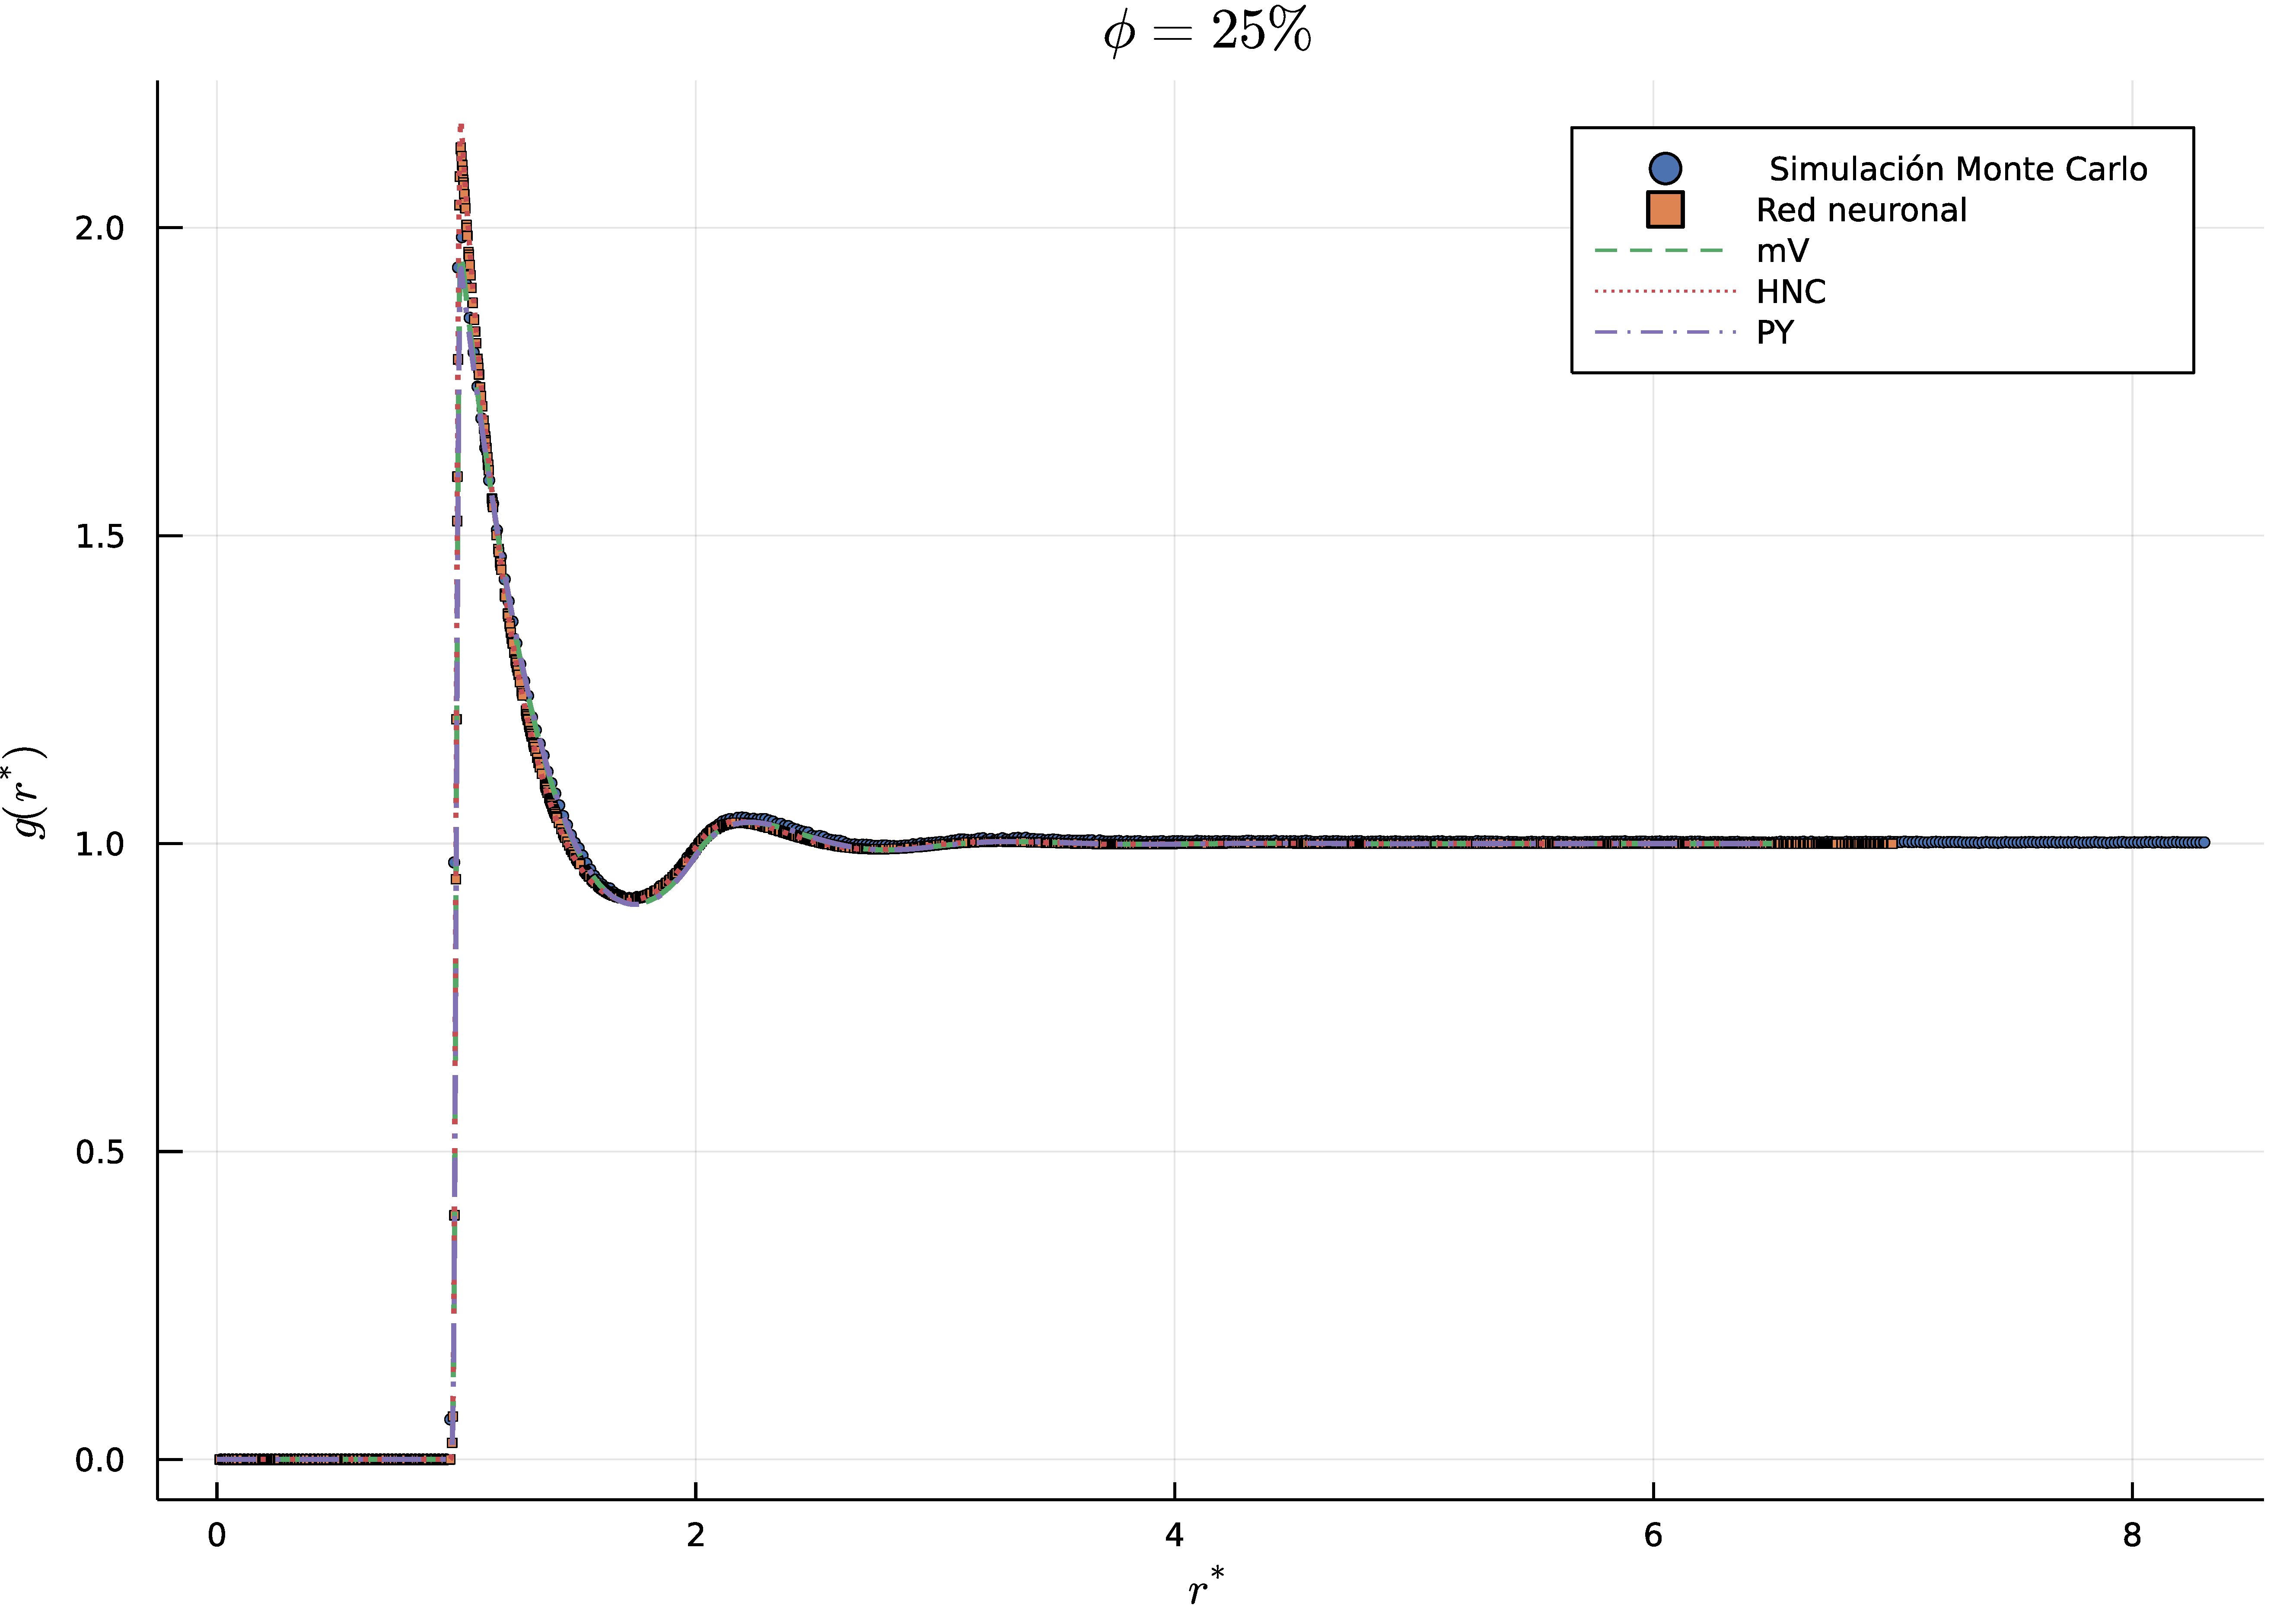
\includegraphics[width=\textwidth]{figuras/capitulo-3/p=0.25.pdf}
    \caption{Una figura.}
    \label{fig:fig2}
\end{figure}

\begin{figure}
    \centering
    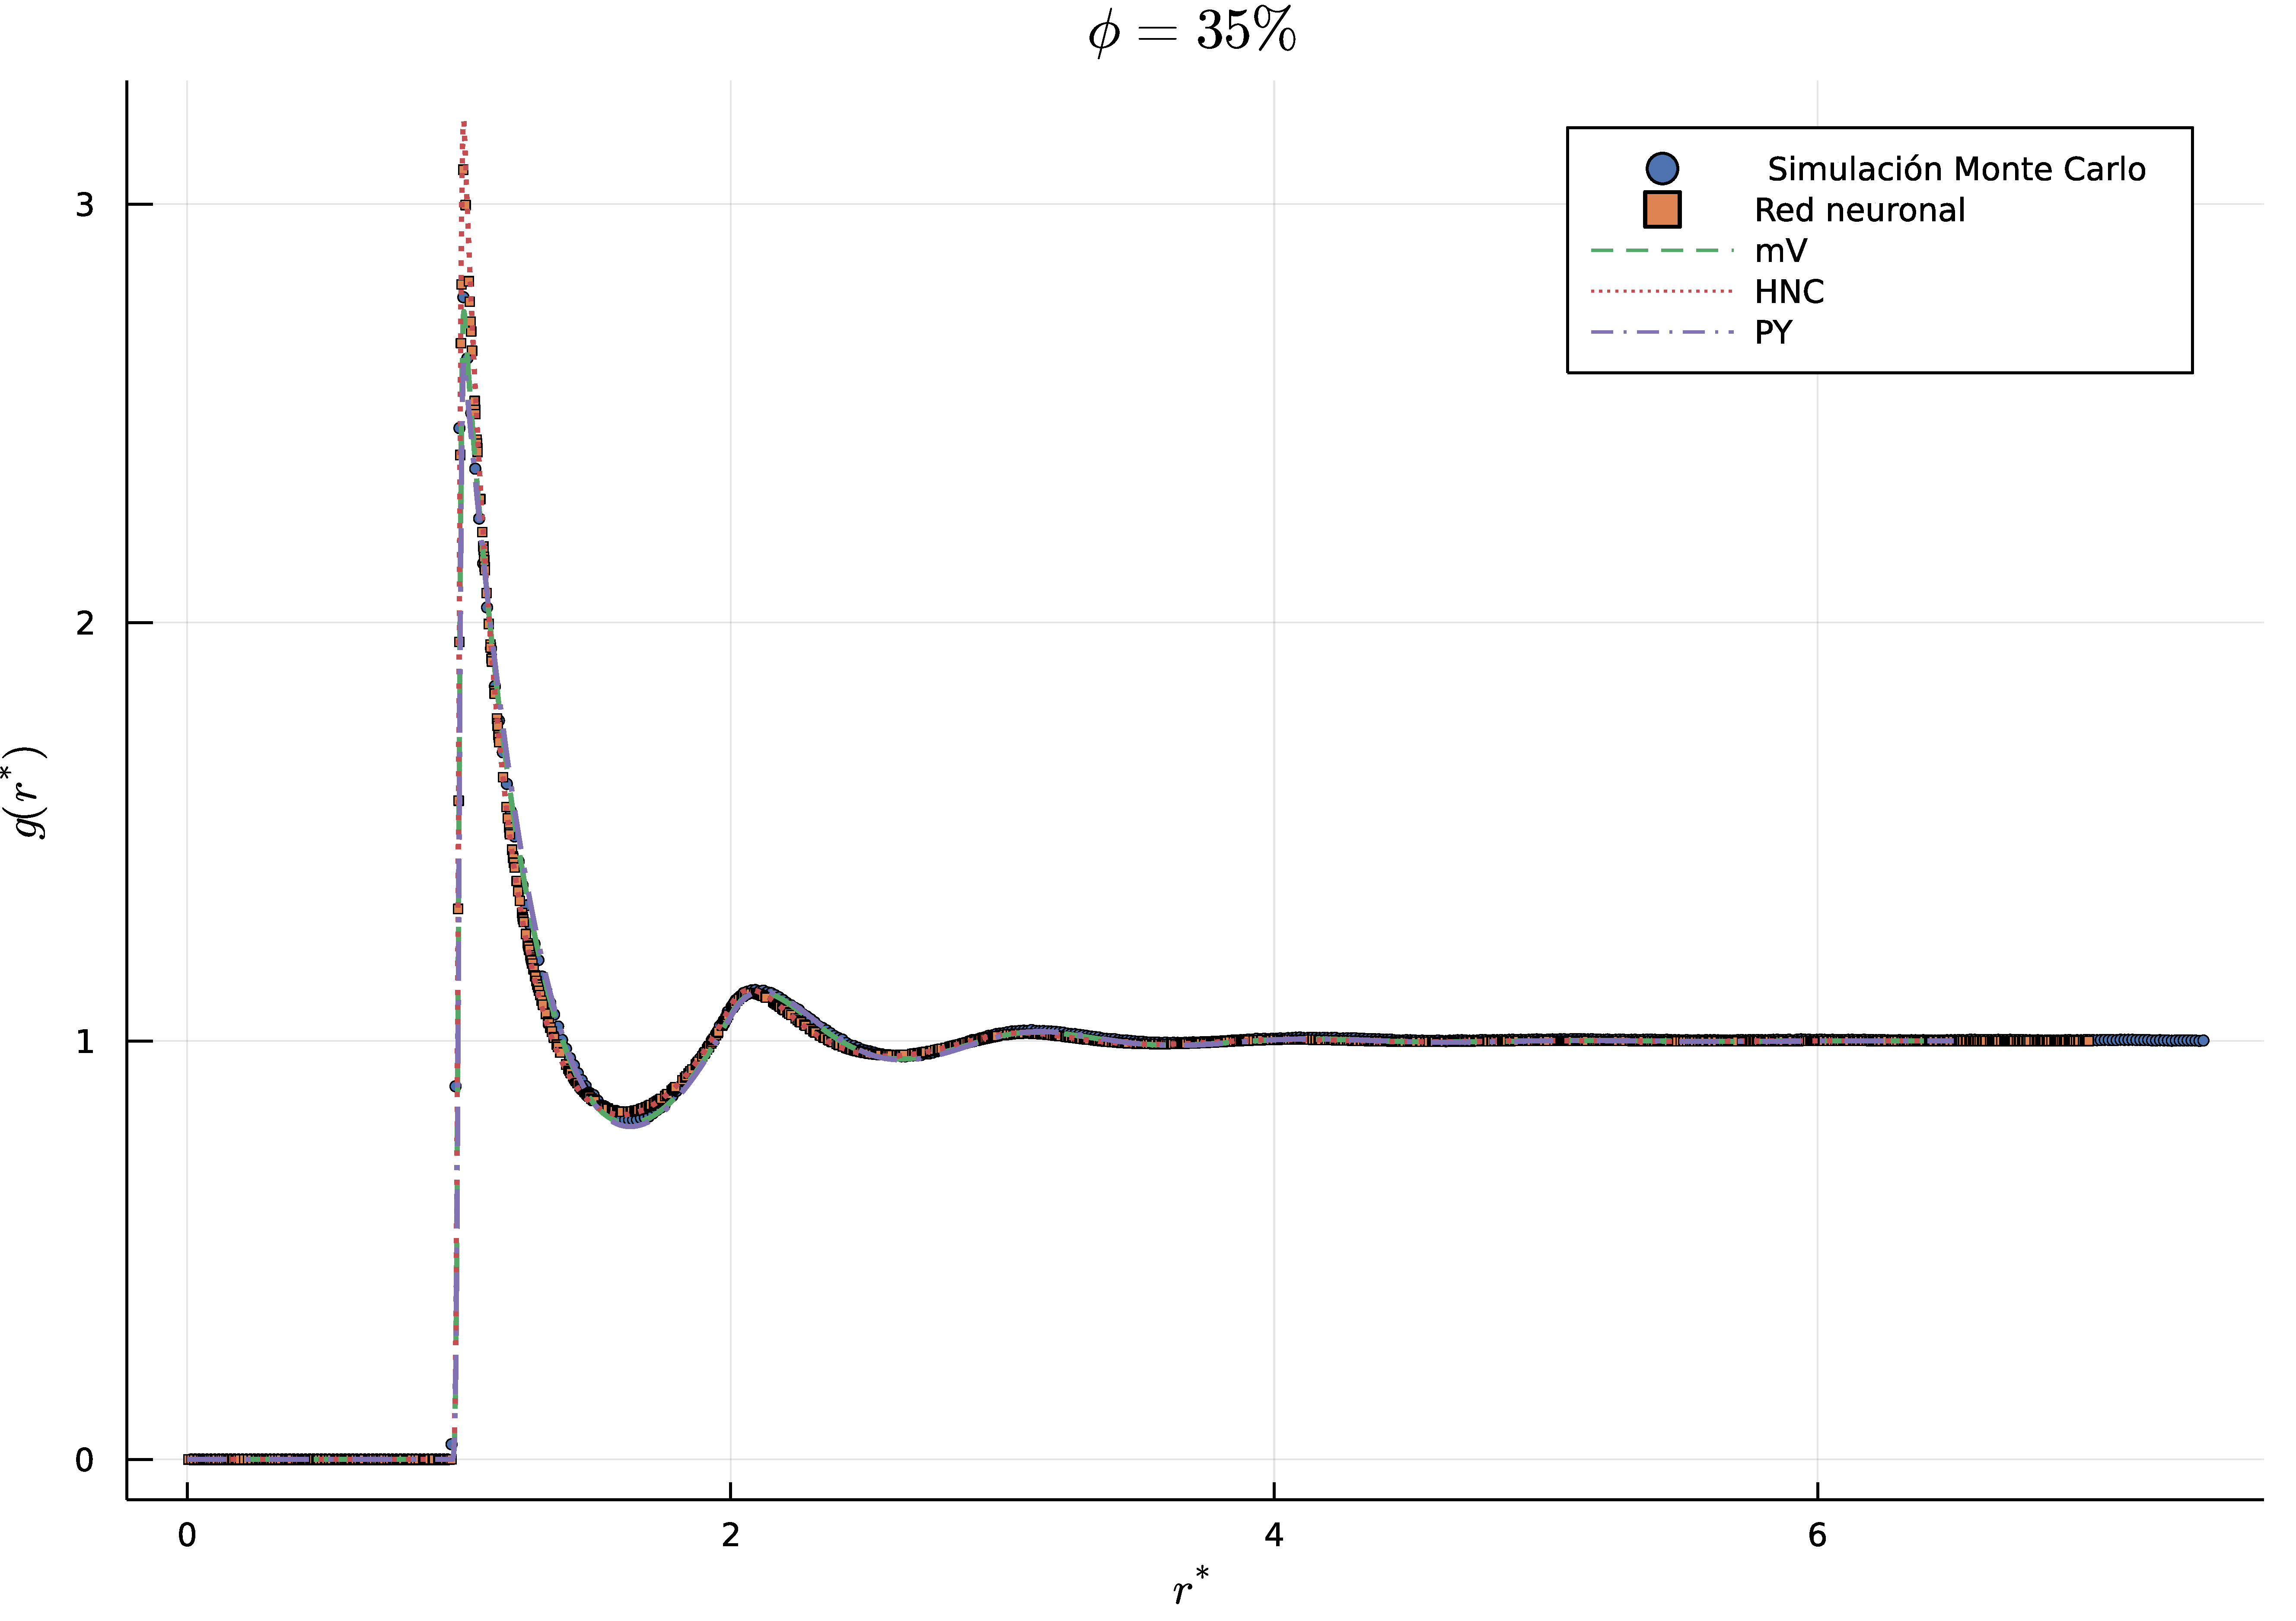
\includegraphics[width=\textwidth]{figuras/capitulo-3/p=0.35.pdf}
    \caption{Una figura.}
    \label{fig:fig3}
\end{figure}

\begin{figure}
    \centering
    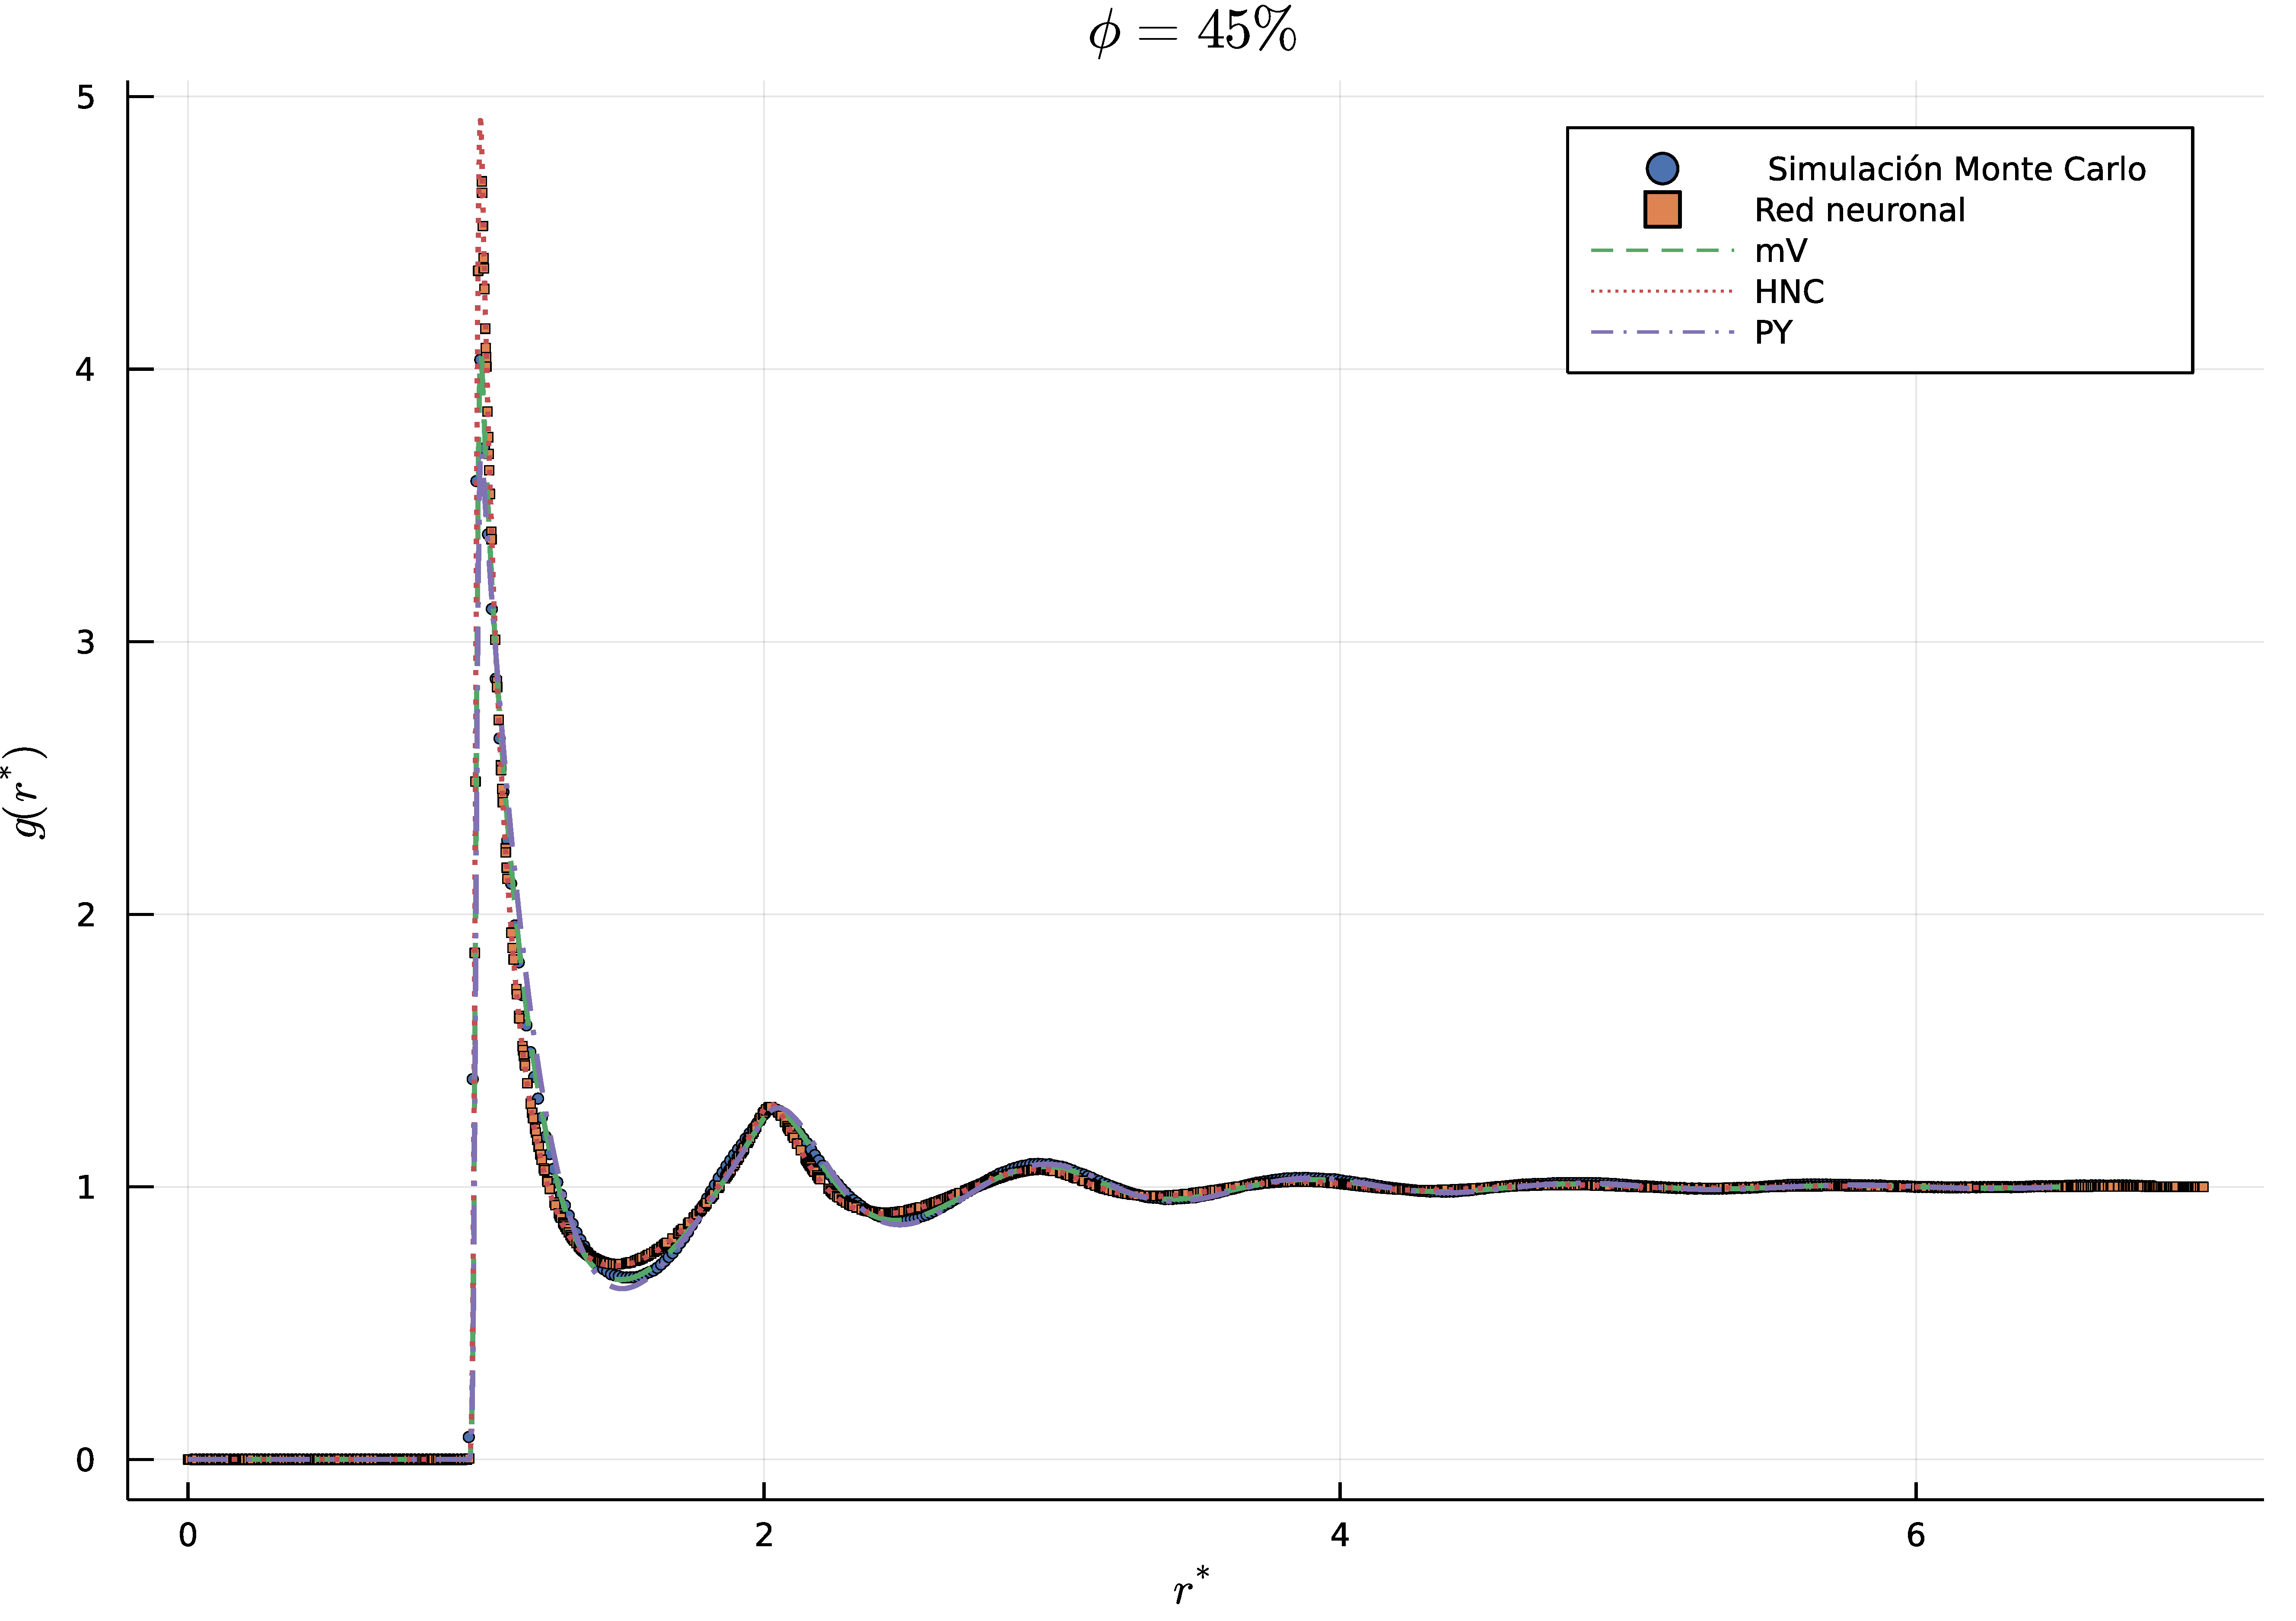
\includegraphics[width=\textwidth]{figuras/capitulo-3/p=0.45.pdf}
    \caption{Una figura.}
    \label{fig:fig4}
\end{figure}
